% easychair.tex,v 3.5 2017/03/15
\PassOptionsToPackage{x11names}{xcolor}

\documentclass{easychair}
%\documentclass[EPiC]{easychair}
%\documentclass[EPiCempty]{easychair}
%\documentclass[debug]{easychair}
%\documentclass[verbose]{easychair}
%\documentclass[notimes]{easychair}
%\documentclass[withtimes]{easychair}
%\documentclass[a4paper]{easychair}
%\documentclass[letterpaper]{easychair}

%------------------------------------------------------------------------------
%% DRAFT options
%\usepackage{lineno}
%\linenumbers

\usepackage{todonotes}
%% \setuptodonotes{inline}
%------------------------------------------------------------------------------

\usepackage{catchfilebetweentags}
\makeatletter

\newrobustcmd*\OrigExecuteMetaData[2][\jobname]{%
\CatchFileBetweenTags\CatchFBT@tok{#1}{#2}%
\global\expandafter\CatchFBT@tok\expandafter{%
\expandafter}\the\CatchFBT@tok
}%\OrigExecuteMetaData

\newrobustcmd*\ChkExecuteMetaData[2][\jobname]{%
\CatchFileBetweenTags\CatchFBT@tok{#1}{#2}%
\edef\mytokens{\detokenize\expandafter{\the\CatchFBT@tok}}
\ifx\mytokens\empty\PackageError{catchfilebetweentags}{the tag #2 is not found\MessageBreak in file #1 \MessageBreak called from \jobname.tex}{use a different tag}\fi%
}%\ChkExecuteMetaData

\renewrobustcmd*\ExecuteMetaData[2][\jobname]{%
\ChkExecuteMetaData[#1]{#2}%
\OrigExecuteMetaData[#1]{#2}%
}

\makeatother

\usepackage{idris2}

\usepackage{doc}
\usepackage{wrapfig}

% use this if you have a long article and want to create an index
% \usepackage{makeidx}

% In order to save space or manage large tables or figures in a
% landcape-like text, you can use the rotating and pdflscape
% packages. Uncomment the desired from the below.
%
% \usepackage{rotating}
% \usepackage{pdflscape}

\usepackage{amsfonts}


\usepackage{tikz}
\usetikzlibrary{automata, positioning, arrows}
\tikzset{
  ->, % makes the edges directed
  >=stealth', % makes the arrow heads bold
  node distance=2.5cm, % specifies the minimum distance between two nodes. Change if necessary.
  every state/.style={thick, fill=gray!10, minimum size=1cm}, % sets the properties for each ’state’ node
  initial text=$ $, % sets the text that appears on the start arrow
}

%% Front Matter
%%
% Regular title as in the article class.
%
\title{Type-safe Bidirectional Channels in Idris 2}

% Authors are joined by \and. Their affiliations are given by \inst, which indexes
% into the list defined using \institute
%
\author{Guillaume Allais\inst{1}}

% Institutes for affiliations are also joined by \and,
\institute{
  University of Strathclyde,
  Glasgow, Scotland, United Kingdom\\
  \email{guillaume.allais@strath.ac.uk}}

%  \authorrunning{} has to be set for the shorter version of the authors' names;
% otherwise a warning will be rendered in the running heads. When processed by
% EasyChair, this command is mandatory: a document without \authorrunning
% will be rejected by EasyChair

\authorrunning{Guillaume Allais}

% \titlerunning{} has to be set to either the main title or its shorter
% version for the running heads. When processed by
% EasyChair, this command is mandatory: a document without \titlerunning
% will be rejected by EasyChair
\titlerunning{Type-safe Bidirectional Channels in Idris 2}

\begin{document}

\maketitle

%------------------------------------------------------------------------------
\subsection*{Introduction}

Session types are a channel typing discipline ensuring that the
communication patterns of concurrent programs abide by a shared
protocol.
%
A meta-theoretical analysis of the typing discipline can then
ensure that the communicating processes will have good properties
e.g. deadlock-freedom.
%
We show how to use a linear dependently typed programming language
to define a direct and type-safe embedding of expressive binary
session types.

%------------------------------------------------------------------------------
\subsection*{Expressive Session Types}

\newcommand{\nat}{\ensuremath{\mathbb{N}}}
\newcommand{\str}{\ensuremath{\mathbb{S}}}
\newcommand{\recvar}[1]{\ensuremath{\mathit{#1}}}
\newcommand{\send}[2]{\ensuremath{!#1.~#2}}
\newcommand{\recv}[2]{\ensuremath{?#1.~#2}}
\newcommand{\select}[2]{\ensuremath{#1 \mathop{\oplus} #2}}
\newcommand{\offer}[2]{\ensuremath{#1 \mathop{\&} #2}}
\newcommand{\smallest}[2]{\ensuremath{\mu #1.~#2}}
\newcommand{\largest}[2]{\ensuremath{\nu #1.~#2}}
\newcommand{\stopsesh}{\ensuremath{\mathtt{end}}}

\noindent
\begin{wrapfigure}[25]{r}{.38\textwidth}\centering%
  \vspace{-1cm}%
  \begin{align*}%
  p,~ q,~ \dots &
    \; ::= \; \recvar{x}
    \; | \; \smallest{x}{p}
    \; | \; \largest{x}{p} \\
    &
    \; | \; \send{A}{p}
    \; | \; \recv{A}{p}
    \; | \; \stopsesh{} \\
    &
    \; | \; \offer{p}{q}
    \; | \; \select{p}{q}
  \end{align*}

  \vspace{.4cm}

  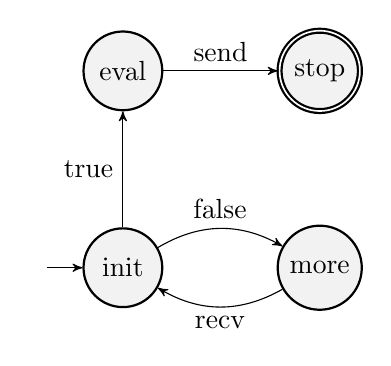
\begin{tikzpicture}
    \node[state, initial]                     (q1)  {init};
    \node[state, above of=q1] (q2r) {eval};
    \node[state, right of=q1]                (q2l) {more};
    \node[state, accepting, right of=q2r]     (q3)  {stop};
    \draw
      (q1) edge[bend left, above]  node{false}       (q2l)
      (q1) edge[left]      node{true}       (q2r)
      (q2l) edge[bend left, below] node{recv \nat} (q1)
      (q2r) edge[above]            node{send \nat} (q3);
  \end{tikzpicture}

  \vspace{.4cm}

  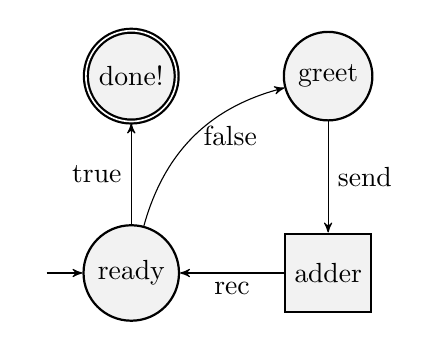
\begin{tikzpicture}
    \node[state, initial]                      (o1)  {ready};
    \node[state, above of=o1, accepting] (o2)  {done!};
    \node[state, right of=o2] (o3)  {greet};
    \node[state, shape=rectangle, below of=o3] (q1)  {adder};
    \draw
      (o1) edge[bend left, right] node{false} (o3)
      (o1) edge[left]            node{true}  (o2)
      (o3) edge[right] node{send \str} (q1)
      (q1) edge[below] node{rec}   (o1);
  \end{tikzpicture}
\end{wrapfigure}
%
Our session types are closed under
nested smallest (\smallest{x}{\cdot}) and largest (\largest{x}{\cdot}) fixpoints,
typed sends (\send{A}{\cdot}) and receives (\recv{A}{\cdot}),
the empty protocol (\stopsesh{})
and branch offerings (\offer{\cdot}{\cdot}) and selections (\select{\cdot}{\cdot}).

The session
$
\largest{i}{(\offer
  {(\send{\nat}{\stopsesh})}}
  {(\recv{\nat}{\recvar{i}}))}
$
types a server for the ``adder'' protocol represented as
a finite state machine on the right hand side.
%
The server accepts an arbitrarily long sequence of natural numbers
(sent by a client repeatedly selecting the
\emph{more} = (\recv{\nat}{\recvar{x}}) branch)
before sending back their sum as a single number
(when the \emph{eval} = (\send{\nat}{\stopsesh}) branch is ultimately selected)
and terminating.
%
The encoding of the server's type uses a largest fixpoint
because the client is the one responsible
for ensuring the process terminates by eventually selecting
the \emph{eval} branch.

We can use nested fixpoint to describe more complex
protocols. For instance, the session described by
$
\largest{r}{(\offer{\stopsesh}
  {(\send{\str}{\largest{i}{(\offer
  {(\send{\nat}{\recvar{r}})}}
  {(\recv{\nat}{\recvar{i}}))}}
  ))})}
$
informally corresponds to the finite state machine
shown on the right hand side.
%
It types a server repeatedly offering to handle the adder
protocol described above after greeting the user with a string.
We replaced adder's \stopsesh{} with \recvar{r} to let the protocol
loop back to the ``ready'' state once the adder is done.


%------------------------------------------------------------------------------
\subsection*{Type-safe Implementation}

\paragraph{Pairs of Unityped Channels}
We represent a bidirectional channel parametrised by a session
type as a pair of unityped unidirectional channels.
%
The key idea behind this safe implementation is to collect
all the received (respectively sent) types used in a protocol
and to manufacture a big sum type in which we can inject all
of the received (respectively sent) values.
%
Because the received types of a protocol are equal to the sent
types of its dual (and vice-versa), we can prove that the directed
channels of two communicating parties are indeed type-aligned.
%
The definition of this sum type is a type safe realisation of
Kiselyov and Sabry's open union type~\cite{DBLP:conf/haskell/KiselyovSS13}
using the encoding of scope-safe
De Bruijn indices~\cite{MANUAL:journals/math/debruijn72}
introduced by Brady in Idris 2's core~\cite{DBLP:conf/ecoop/Brady21}.
%
We include below its definition: given
a list \IdrisBound{ts} of values of type \IdrisBound{a}
and a decoding function \IdrisBound{elt} turning such values into types,
\IdrisType{UnionT} defines a union type characterised by its one
constructor \IdrisData{Element}.
\IdrisData{Element} takes a natural number \IdrisBound{k} functioning as a tag,
a proof that the value \IdrisBound{t} is present at index \IdrisBound{k}
in \IdrisBound{ts} and injects a value of type (\IdrisBound{elt} \IdrisBound{t})
into the union type.
%
By picking \IdrisBound{elt} to be the identity function, we recover the
usual notion of union of types

\ExecuteMetaData[Data/OpenUnion/PrintOnly.idr.tex]{uniont}
%\ExecuteMetaData[Data/OpenUnion/PrintOnly.idr.tex]{union}

Note that the proof of type
(\IdrisType{AtIndex} \IdrisBound{t} \IdrisBound{ts} \IdrisBound{k})
is marked as erased through the use of the \IdrisKeyword{0}
quantity which means this compiles down to a pair of a
GMP-style \IdrisType{Integer} (the optimised runtime representation of \IdrisType{Nat})
and a value of the appropriate type.
%
This gives us an encoding that has constant time injections
and partial projections (via an equality check on the \IdrisType{Nat} tag)
in and out of the big sum type.

\paragraph{Dealing with Changing Sessions}
The session type, by design, changes after each communication
but the big sum type used when communicating across the
unityped channels needs to stay the same.
%
Our solution is to record an offset remembering where we currently
are in the protocol and thus allowing us to keep injecting values to
be sent into the initial shared sum type.
%
Our offsets are proven correct using a gadget that can be understood
as a cut down version of McBride's one hole
contexts~\cite{DBLP:conf/popl/McBride08}. Instead
of recording the full path followed by our programs in the finite
state machine describing the protocol,
we merely record a de-looped version.

\paragraph{Types of the Primitives} We include code snippets showing the
types of the primitives dealing with communications. Note that the Idris~2's
funny arrow (\IdrisFunction{-@}) denotes a linear function space, and
consequently all of these primitives are linear in the channel
they take as an input (ensuring it cannot be reused now that the protocol
has been stepped) and systematically return, wrapped in a linear IO
monad called \IdrisFunction{IO1}, a channel indexed by the updated protocol.
%
First, \IdrisFunction{send} and \IdrisFunction{recv}, the primitives
dealing with sending arbitrary values back and forth.
\IdrisFunction{send} takes an argument of type \IdrisBound{ty} while
\IdrisFunction{recv} returns one as the \IdrisType{Res}ult of the
communication.
%
\ExecuteMetaData[System/Concurrency/Session/MuNuN.idr.tex]{sendrecv}
%
Second, \IdrisFunction{offer} and \IdrisFunction{select}, the primitives
dealing with branching.
%
Both involve a choice in the form of a \IdrisType{Bool} named \IdrisBound{b}
and used to compute the new state of the channel.
%
\IdrisFunction{offer} gets it from the other thread as a \IdrisType{Res}ult
of some communication while \IdrisFunction{select} requires the caller to
pass it and will forward the decision to the other party.
%
\ExecuteMetaData[System/Concurrency/Session/MuNuN.idr.tex]{offerselect}
%
Third, \IdrisFunction{unroll} and \IdrisFunction{roll}, the
primitives dealing with the iso-recursive nature of our
(co)inductive protocols.
%
The type of these primitives reveal the role of \IdrisType{Channel}'s
second parameter: it is a stack of open session types corresponding
to the bodies of the nested fixpoints encountered during execution.
%
\IdrisFunction{unroll} opens a fixpoint and thus pushes a new entry onto the
stack \IdrisBound{e} while \IdrisFunction{roll} does the opposite.
\ExecuteMetaData[System/Concurrency/Session/MuNuN.idr.tex]{unrollroll}
%
Last but not least, \IdrisFunction{rec} steps a channel that has
reached a recursive call to a fixpoint by looking up the
open session and environment associated to the specified
\IdrisBound{pos}ition in the stack and reinstating them.
\ExecuteMetaData[System/Concurrency/Session/MuNuN.idr.tex]{rec}

\paragraph{Example Server} Omitting the somewhat horrifying types,
we include the implementation of the server repeatedly offering
to greet the user and execute the adder protocol that we sketched
earlier.
%
We use Idris~2's named argument syntax to explicitly pass the name
\IdrisBound{nm} to the \IdrisFunction{unroll} and \IdrisFunction{rec}
calls in order to clarify what step of the protocol is being reached.

\noindent\begin{minipage}[t]{.49\textwidth}
  \ExecuteMetaData[System/Concurrency/Session/MuNuN.idr.tex]{server}
\end{minipage}\hfill
\begin{minipage}[t]{.49\textwidth}
  \ExecuteMetaData[System/Concurrency/Session/MuNuN.idr.tex]{adder}
\end{minipage}

On the left hand side we are acting as a server parametrised by a client
\IdrisBound{id} number. We \IdrisFunction{unroll} the largest fixpoint
corresponding to the `ready' state repeatedly offering the adder protocol,
and wait for the client to choose one of the branches we \IdrisFunction{offer}.
If they are done we \IdrisFunction{close} the channel and terminate,
otherwise we \IdrisFunction{send} a greeting and call the
\IdrisFunction{adder} with an accumulator initialised to \IdrisData{0},
and eventually continue acting as the server with an increased client id number.

One the right hand side we are acting as the adder parametrised by an
accumulator \IdrisBound{acc}. We \IdrisFunction{unroll} the largest
fixpoint corresponding to the ``adder'' protocol and immediately
\IdrisFunction{offer} the client a choice between getting the current
running total or sending us more numbers.
%
If they are done, we \IdrisFunction{send} back the value in the accumulator
and, having reached a \IdrisData{Rec} variable, use \IdrisFunction{rec} to
jump back to the ``ready'' state.
%
Otherwise we \IdrisFunction {recv} an additional number,
add it to the accumulator and continue as \IdrisFunction{adder}.

%------------------------------------------------------------------------------
\subsection*{Limitations and Future Work}

\paragraph{Encoding Uniqueness via Linear Types}
Unlike Brady's prior work in Idris 1~\cite{DBLP:journals/aghcs/Brady17},
we are using Idris 2 which does not currently have uniqueness types.
We are forced to use the linearity granted to us by
Quantitative Type Theory (QTT)~\cite{DBLP:conf/birthday/McBride16,DBLP:conf/lics/Atkey18}
to emulate uniquess via a library-wide invariant.
%
This adds a degree of noise and trust to the implementation.
We would ideally want a system combining both linearity and uniqueness
to benefit from enhanced expressivity and efficiency as described
by Marshall, Vollmer, and Orchard~\cite{DBLP:conf/esop/MarshallVO22}.

\paragraph{Small Runtime Overhead}
In the current version of our library, we compute a handful
of key offset values by induction over the protocol. Correspondingly
the protocol is not marked as erased anymore and, if compilation does
not specialise the relevant combinators agressively, then we may very
well be evaluating these relatively small computations at runtime.
%
As far as we understand, directly adding typed staging to Idris 2
through the use of a two-level type theory à la
Kov{\'{a}}cs~\cite{DBLP:journals/pacmpl/Kovacs22} would not be
enough to solve our issue: for typing purposes, the protocol does need
to persist through staging. But it should be possible to move it
from QTT's unrestricted to its erased modality.

\paragraph{Ergonomics}
We found writing the types of inner loops of programs with non-trivial
communication patterns to be tedious as they expose quite a lot of the
powerful but noisy encoding of syntaxes with binding we use.
Figuring out a more user-friendly surface syntax for our protocols is
left as future work.




%------------------------------------------------------------------------------
%% BIBLIOGRAPHY

\newpage
\bibliographystyle{plain}
%\bibliographystyle{alpha}
%\bibliographystyle{unsrt}
%\bibliographystyle{abbrv}
\bibliography{session}

\end{document}
